\lab{Total Variation and Image Processing}{Total Variation and Image Processing}
\label{lab:tv_images}
\objective{Minimizing an energy functional is equivalent to solving the resulting Euler-Lagrange equations.  We introduce the method of steepest descent to solve these equations, and apply this technique to a denoising problem in image processing.}



% \begin{enumerate}
% \item Algorithm assumes smoothness.
% Other theorems/algorithms have been developed using convex analysis, due to the recognition that the image might not be best represented by a smooth function $u:[0,1]\times [0,1] \to \mathbb{R}$.
% \item Analyze efficiency.
% Code with cython/numexpr?
% \end{enumerate}

\section*{The Gradient Descent method}
Consider an energy functional $E[u]$, defined over a collection of admissible functions $u:\Omega \subset \mathbb{R}^n \to \mathbb{R}$. 
We suppose the energy functional $E$ has the form 
\[E[u] = \int_{\Omega} L(x,u,\nabla u) \, dx\]
where $L = L(x,y,w)$ is a function $\mathbb{R}^n \times \mathbb{R} \times \mathbb{R}^n \to \mathbb{R}$. 
A standard result from the calculus of variations states that a minimizing function $u^*$ satisfies the Euler-Lagrange equation
\begin{align}
L_y - {\rm div}\,(L_w) &= 0.	\label{EL:multivar_domain}
\end{align}

This equation is typically an elliptic PDE, possessing boundary conditions associated with  restrictions on the class of admissible functions $u$.
To more easily compute $\eqref{EL:multivar_domain}$, we may consider a related parabolic PDE:
\begin{align}
	\begin{split}
	&{ } u_t = -(L_y - {\rm div}\, L_w),\\
	&{ } u(x,t=0) = u_0(x).
	\end{split} \label{grad_desc_pde}
\end{align}
A steady state solution of \eqref{grad_desc_pde} does not depend on time, and thus is a solution of the Euler-Lagrange equation. 
In practice, it is often easier to evolve an initial guess $u_0$ using \eqref{grad_desc_pde}, stopping whenever its steady state is well-approximated, then to solve \eqref{EL:multivar_domain} directly. 

\begin{example}
Consider the energy functional 
\[ E[u] = \int_{\Omega} \|\nabla u\|^2 \, dx,\]
where the class of admissible functions $u$ satisfy appropriate Dirichlet conditions on $\partial \Omega$. 
The minimizing function $u^*$ satisfies the Euler-Lagrange equation
\[-{\rm div}\, \nabla u	= - \triangle u = 0.\]
The related PDE (called the gradient descent flow) is the well-known equation
\[u_t = \triangle u\]
describing heat flow.
\end{example}

The previous example brings to mind an interesting question: The Euler-Lagrange equation could equivalently be described as $\triangle u = 0$, leading to the PDE $u_t = -\triangle u$. 
Since this (backward) heat equation is ill-posed, it will not be helpful in our search for a steady-state. 

Let us take the time to put \eqref{grad_desc_pde} on a more rigorous footing. 
Recalling the derivation of the Euler-Lagrange equation, we note that 
\begin{align*}
		\delta E(u;v) &= \left.\frac{d}{dt}E(u + tv)\right|_{t=0},\\
		&= \int_{\Omega} (L_y(u) - {\rm div}\, L_w(u)) v\, dx
\end{align*}
for each $u$ and each admissible perturbation $v$.
We can now employ the Cauchy-Schwarz inequality: 
\begin{align*}
	|\delta E(u;v)| &= | \langle L_y(u) - {\rm div}\, L_w(u), v \rangle_{L^2(\Omega)} |,\\
	&\leq \|L_y(u) - {\rm div}\, L_w(u)\| \cdot \| v \|,
\end{align*}
with equality iff $v =\alpha u$ for some $\alpha \in \mathbb{R}$. 
This implies that the ``direction" 
$v = L_y(u) - {\rm div}\, L_w(u)$
maximizes $\delta E(u)$. 
Similarly,
\[v = -(L_y(u) - {\rm div}\, L_w(u))\]
 points in the direction of steepest descent, and the flow described by \eqref{grad_desc_pde} tends to move toward a state of lesser energy. 


\subsection*{Example: Finding the curve that surface of revolution minimizes surface area}
Consider the collection of smooth curves defined on $[a,b]$, with fixed end points $y(a) = y_a$, $y(b) = y_b$. The surface obtained by revolving a curve $y(x)$ about the $x$-axis has area given by the functional 
\[A[y] = \int_a^b 2 \pi y \sqrt{1 + (y')^2} \, dx.
\]
The Euler-Lagrange equation is 
\begin{align}
	\begin{split}
	0 &= 1 - y \frac{y''}{1 + (y')^2} , \\
	&= 1 + (y')^2 - y y'',
	\end{split}\label{tv_images:SA_EL_equation}
\end{align}
and the resulting gradient descent flow is given by
\begin{align}
	\begin{split}
	&{ } u_t = -1 - (y')^2 + y y'', \\
	&{ } u(a,t) = y_a, \quad u(b,t) = y_b,\\
	&{ } u(x,0) = g(x),
	\end{split}\label{tv_images:SA_flow}
\end{align}
where $g(x)$ is an appropriate initial guess.

Consider a second-order order discretization in space, with a simple forward Euler step in time. Let us impose the conditions $y(-1) = 1$, $y(1) = 7$. We begin by creating a grid to approximate the solution on: 
\begin{lstlisting}
import numpy as np

a, b = -1, 1.
alpha, beta = 1., 7.
####  Define variables x_steps, final_T, time_steps  ####
delta_t, delta_x = final_T/time_steps, (b-a)/x_steps
x0 = np.linspace(a,b,x_steps+1)
\end{lstlisting}

Often there is a stability condition required for a numerical scheme. 
One that is common for this discretization is that $\frac{\triangle t}{(\triangle x)^2} \leq \frac{1}{2}$.  
We continue by checking that this condition is satisfied, and setting our initial guess to be the straight line connecting the end points. 

\begin{lstlisting}
# Check a stability condition for this numerical method
if delta_t/delta_x**2. > .5:
	print "stability condition fails"
	
u = np.empty((2,x_steps+1))
u[0]  = (beta - alpha)/(b-a)*(x0-a)  + alpha
u[1] = (beta - alpha)/(b-a)*(x0-a)  + alpha
\end{lstlisting}

Finally, we define the right hand side of our difference scheme, and time step until we 
achieve a desired accuracy. 
\begin{lstlisting}
def rhs(y):
	# Approximate first and second derivatives to second order accuracy.
	yp = (np.roll(y,-1) - np.roll(y,1))/(2.*delta_x)
	ypp = (np.roll(y,-1) - 2.*y + np.roll(y,1))/delta_x**2.
	# Find approximation for the next time step, using a first order Euler step
	y[1:-1] -= delta_t*(1. + yp[1:-1]**2. - 1.*y[1:-1]*ypp[1:-1])


# Time step until successive iterations are close
iteration = 0
while iteration < time_steps:
	rhs(u[1])
	if norm(np.abs((u[0] - u[1]))) < 1e-5: break
	u[0] = u[1]
	iteration+=1

print "Difference in iterations is ", norm(np.abs((u[0] - u[1])))
print "Final time = ", iteration*delta_t
\end{lstlisting}

\begin{figure}
\centering
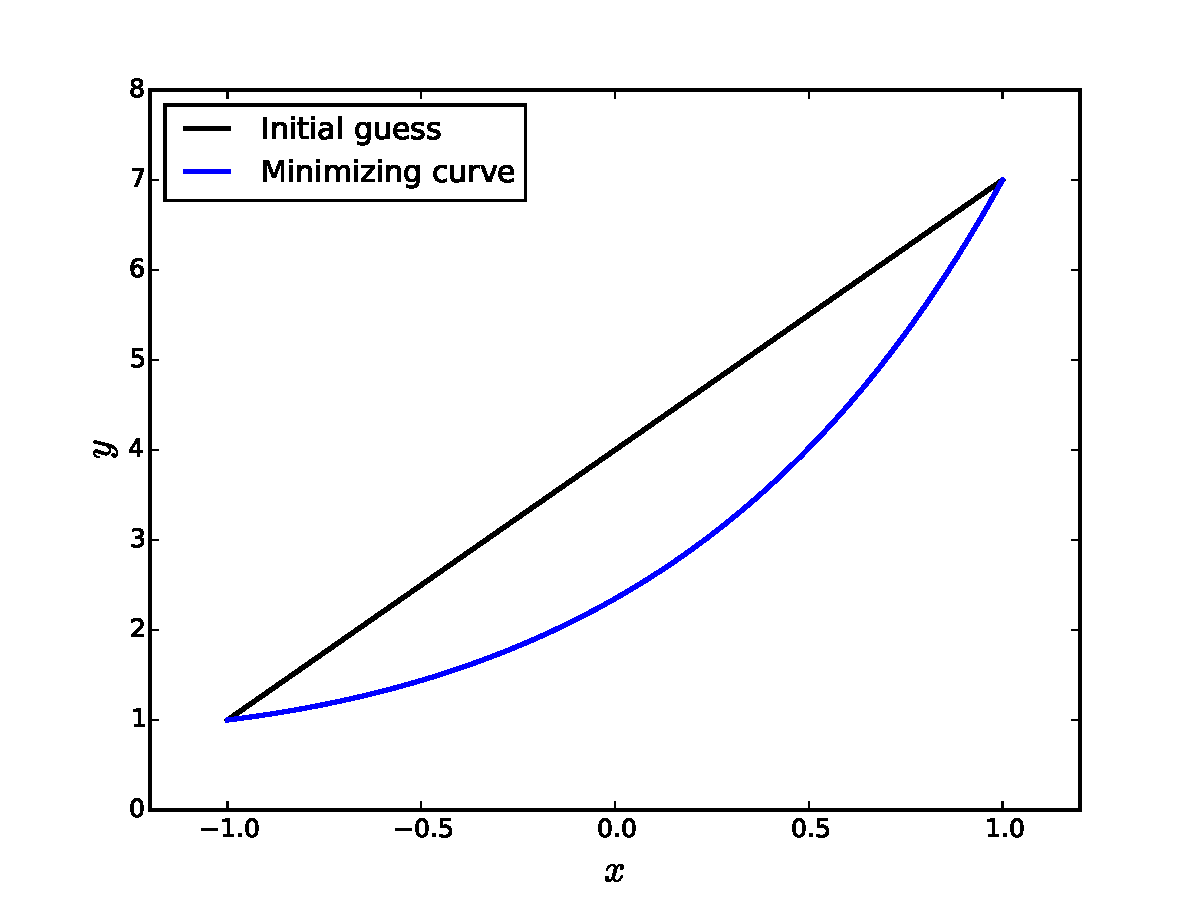
\includegraphics[width=\textwidth]{min_surface_area.pdf}
\caption{The solution of \eqref{tv_images:SA_EL_equation}, found using the gradient descent flow \eqref{tv_images:SA_flow}.}
\label{fig:tv_images:SA_image}
\end{figure}


\section*{Image Processing: A First Attempt}
We represent a (greyscale) image by a function $u:\Omega \to \mathbb{R}$, $\Omega \subset \mathbb{R}^2$. We use the following code to read an image into an array of floating point numbers, add some noise, and save the noisy image: 
\begin{lstlisting}
from numpy.random import random_integers, uniform, randn
import matplotlib.pyplot as plt
from matplotlib import cm
from scipy.misc import imread, imsave

imagename = 'baloons_resized_bw.jpg'
changed_pixels=40000
# Read the image file imagename into an array of numbers, IM
# Multiply by 1. / 255 to change the values so that they are floating point
# numbers ranging from 0 to 1.
IM = imread(imagename, flatten=True) * (1. / 255)
IM_x, IM_y = IM.shape
	
for lost in xrange(changed_pixels):
	x_,y_ = random_integers(1,IM_x-2), random_integers(1,IM_y-2)
	val =  .1*randn() + .5
	IM[x_,y_] = max( min(val,1.), 0.)
imsave(name=("noised_"+imagename),arr=IM)	
\end{lstlisting}
We note that a color image can be represented by three functions $u_1, u_2,$ and $u_3$. In this lab we will work with black and white images, but the techniques can easily be used on more general images. 


Here is our first attempt at denoising: given a noisy image $f$, we look to find a denoised image $u$ minimizing the energy functional 
\begin{align}
E[u] = \int_{\Omega} L(x,\nabla u, u) \, dx, \label{tv_images:diffusion}
\end{align}
where
\begin{align*}
L(x,\nabla u, u) &= \frac{1}{2}(u-f)^2 + \frac{\lambda}{2} | \nabla u|^2,\\
&= \frac{1}{2}(u-f)^2 + \frac{\lambda}{2} (u_x^2 + u_y^2)^2.
\end{align*}
This energy functional penalizes 1) images that are too different from the original noisy image, and 2) images that have a large derivatives. The minimizing denoised image $u$ will balance these two different costs. 

Solving for the original denoised image $u$ is a difficult inverse problem; some information about the image is irretrievably lost when the noise is introduced. A priori information can however be used to guess at the structure of the original image.  For example, in this problem $\lambda$ represents our best guess on how much noise was added to the image. $\lambda$ is known as a regularization parameter in inverse problem theory. 

The Euler-Lagrange equation determined from \eqref{tv_images:diffusion} is
\begin{align*}
L_u - \text{div } L_{\nabla u} &= (u-f) - \lambda \triangle u,\\
&= 0.
\end{align*}
The resulting gradient descent flow is then given by 
\begin{align}
	\begin{split}
u_t &= -(u-f -\lambda \triangle u),\\
u(x,0) &= f(x).	
	\end{split} \label{tv_images:diffusion_flow}
\end{align}

Let $u_{ij}^n$ represent our approximation to $u(x_i,y_j)$ at time $t_n$. We will approximate $u_t$ with a forward Euler difference, and $\triangle u$ with centered differences: 
\begin{align*}
	u_t &\approx \frac{u_{ij}^{n+1}-u_{ij}^n}{\triangle t},\\
	u_{xx} &\approx \frac{u_{i+1,j}^{n}-2u_{ij}^n + u_{i-1,j}^n}{\triangle x^2}, \\
	u_{yy} &\approx \frac{u_{i,j+1}^{n}-2u_{ij}^n + u_{i,j-1}^n}{\triangle y^2}.
\end{align*}


\begin{problem}
Using $\triangle t = 1e-3, \lambda = 40, \triangle x = 1,$ and $ \triangle y = 1$, implement the numerical scheme mentioned above to obtain a solution $u$. (So $\Omega = [0,n_x]\times [0,n_y]$, where $n_x$ and $n_y$ represent the number of pixels in the $x$ and $y$ dimensions, respectively.) Take 250 steps in time. Compare your results with Figure \ref{fig:noise_compare_attempts}.

Hint: use the function \li{np.roll} to compute the spatial derivatives. Consider the following: 
\begin{lstlisting}
u_xx = np.roll(u,-1,axis=0) - 2*u + np.roll(z,1,axis=0)	
\end{lstlisting}
\end{problem}




% diffusion_denoised_baloons_resized_bw.jpg
% \begin{lstlisting}
% delta_t = 1e-3
% lmbda = 40
% u = np.empty((2,IM_x,IM_y))
% u[1] = IM
%
% def laplace(z):
% 	# Approximate first and second derivatives to second order accuracy.
% 	z_xx = (np.roll(z,-1,axis=0) - 2.*z + np.roll(z,1,axis=0))#/delta_x**2.
% 	z_yy = (np.roll(z,-1,axis=1) - 2.*z + np.roll(z,1,axis=1))#/delta_y**2.
% 	# Find approximation for the next time step, using a first order Euler step
% 	z[1:-1,1:-1] -= delta_t*(   (z[1:-1,1:-1]-IM[1:-1,1:-1])
% 									-lmbda*(z_xx[1:-1,1:-1] + z_yy[1:-1,1:-1]))
%
% # Iterate towards a steady state solution of the gradient descent flow.
% iteration = 0
% while iteration < time_steps:
% 	laplace(u[1])
% 	if norm(np.abs((u[0] - u[1]))) < 1e-4: break
% 	u[0] = u[1]
% 	iteration+=1
%
% \end{lstlisting}
\begin{figure}
\begin{minipage}[b]{.47\linewidth}
\centering
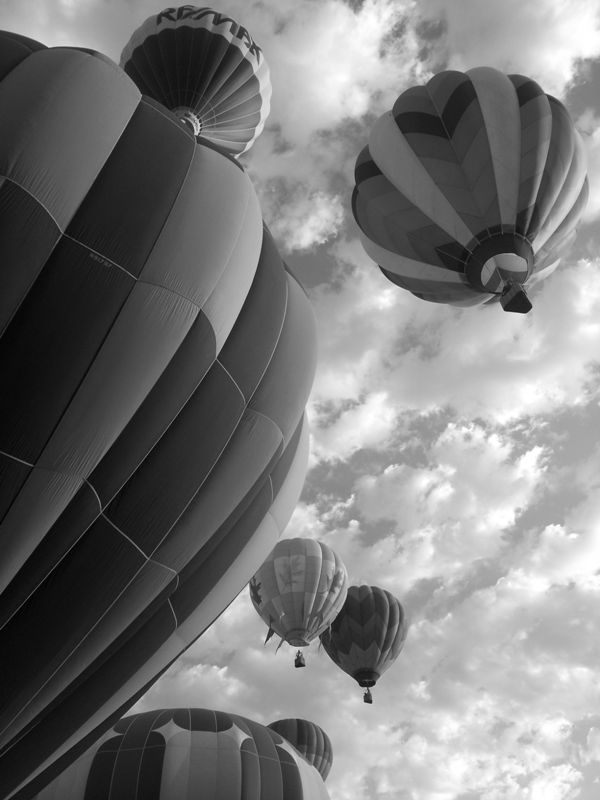
\includegraphics[width=\textwidth]{baloons_resized_bw.jpg}
\caption*{Original image}
\end{minipage}
\hspace{0.5cm}
\begin{minipage}[b]{0.47\linewidth}
\centering
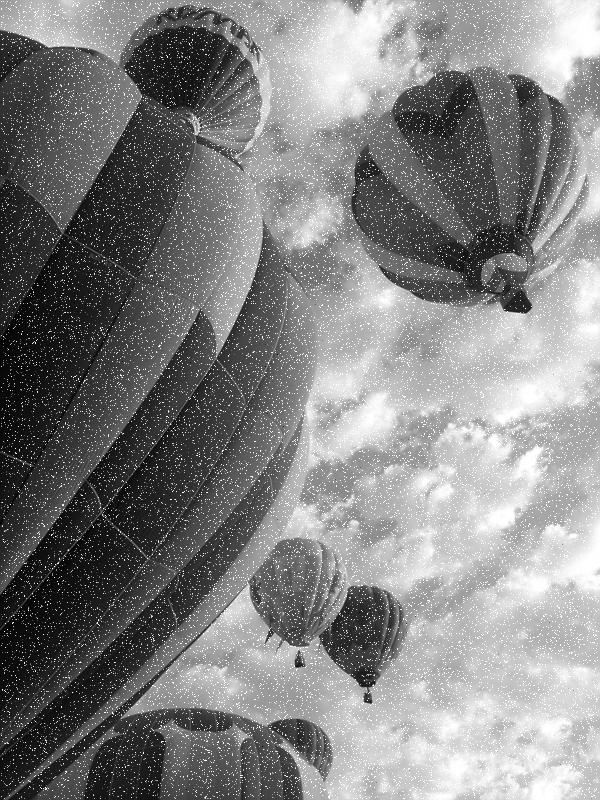
\includegraphics[width=\textwidth]{lab_noised_baloons_resized_bw.jpg}
\caption*{Image with white noise}
\end{minipage}
\caption{Noise.}
\label{fig:noise_firstattempt}
\end{figure}

\begin{figure}
\begin{minipage}[b]{.47\linewidth}
\centering
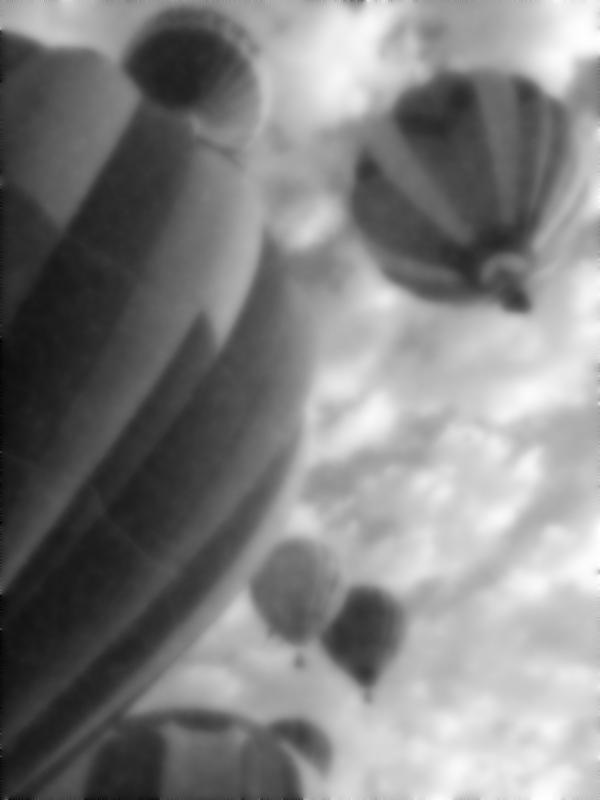
\includegraphics[width=\textwidth]{diffusion_denoised_baloons_resized_bw.jpg}
\caption*{Initial diffusion-based approach}
\end{minipage}
\hspace{0.5cm}
\begin{minipage}[b]{0.47\linewidth}
\centering
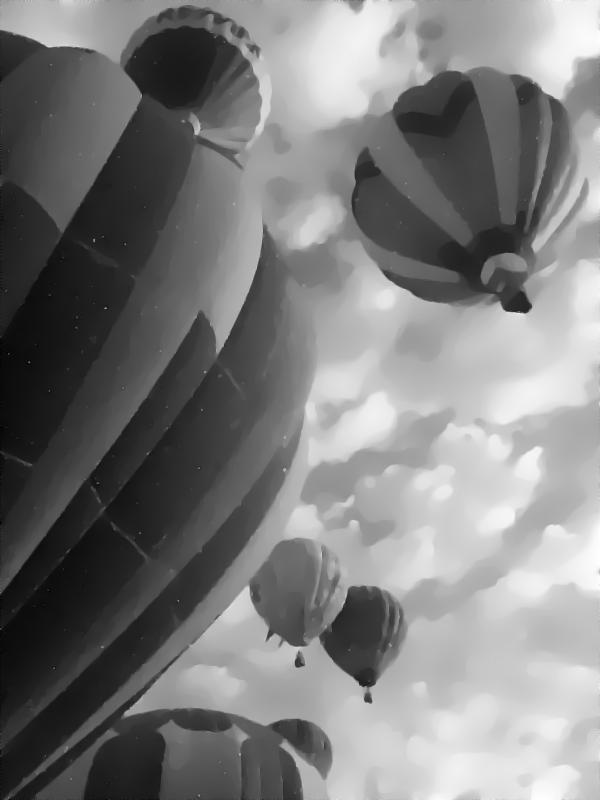
\includegraphics[width=\textwidth]{tv_denoised_baloons_resized_bw.jpg}
\caption*{Total variation based approach}
\end{minipage}
\caption{The solutions of \eqref{tv_images:diffusion_flow} and \eqref{tv_images:tv_flow}, found using a first order Euler step in time and centered differences in space.}
\label{fig:noise_compare_attempts}
\end{figure}

% \begin{figure}
% \centering
% 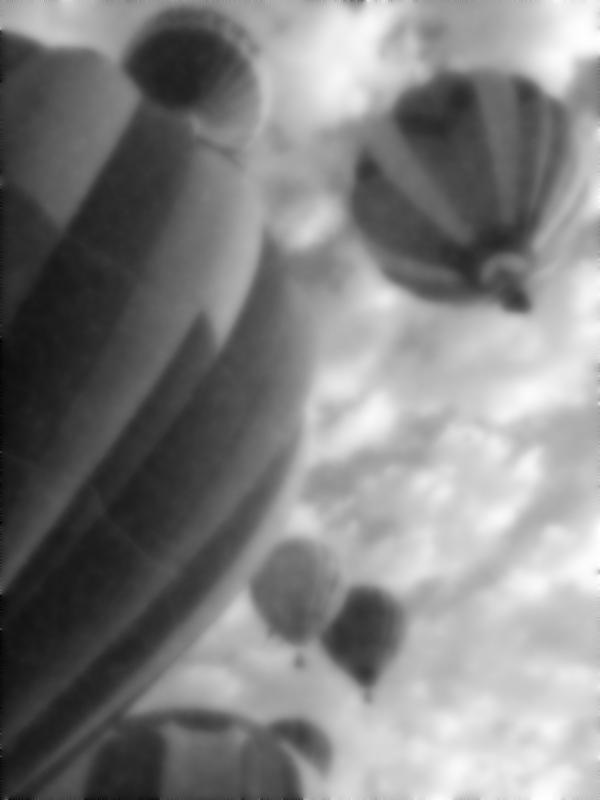
\includegraphics[width=6cm]{diffusion_denoised_baloons_resized_bw.jpg}
% \caption{The solution of \eqref{tv_images:diffusion_flow}, found using a first order Euler step in time and centered differences in space.}
% \label{fig:diffusion_image_denoised}
% \end{figure}

\section*{Image Processing: Total Variation Method}
We represent an image by a function $u:[0,1]\times[0,1] \to \mathbb{R}$. 
A $C^1$ function $u:\Omega \to \mathbb{R}$ has bounded total variation on $\Omega$ ($BV(\Omega)$) if $\int_{\Omega} |\nabla u| < \infty$; $u$ is said to have total variation $\int_{\Omega} |\nabla u|$.  Intuitively, the total variation of an image $u$ increases when noise is added. 

The total variation approach was originally introduced by Ruding, Osher, and Fatemi\footnote{L. Rudin, S. Osher, and E. Fatemi, ``Nonlinear total variation based noise removal algorithms'', \emph{Physica D.}, 1992.}. It was formulated as follows: given a noisy image $f$, we look to find a denoised image $u$ minimizing 
\begin{align}
\int_{\Omega} |\nabla u(x)|\, dx \label{tv_images:tv}
\end{align}
subject to the constraints 
\begin{align}
	&{ } \int_{\Omega} u(x) \, dx = \int_{\Omega} f(x)\, dx, \label{tv_images:same_mean}\\
	&{ } \int_{\Omega} |u(x) - f(x)|^2\, dx = \sigma |\Omega|.\label{tv_images:aprior_variance}
\end{align}
Intuitively, \eqref{tv_images:tv} penalizes fast variations in $f$ - this functional together with the constraint \eqref{tv_images:same_mean} has a constant minimum of $u = \frac{1}{|\Omega|}\int_{\Omega} u(x) \, dx$. This is obviously not what we want, so we add a constraint \eqref{tv_images:aprior_variance} specifying how far $u(x)$ is required to differ from the noisy image $f$.  More precisely, \eqref{tv_images:same_mean} specifies that the noise in the image has zero mean, and \eqref{tv_images:aprior_variance} requires that a variable $\sigma$ be chosen a priori to represent the standard deviation of the noise. 



Chambolle and Lions proved that the model introduced by Rudin, Osher, and Fatemi can be formulated equivalently as 
\begin{align}
F[u] = \min_{u \in BV(\Omega)} \int_{\Omega} |\nabla u| + \frac{\lambda}{2}(u-f)^2 \, dx,	
\end{align}
where $\lambda >0$ is a fixed regularization parameter\footnote{A. Chambelle and P.-L. Lions, ``Image recovery via total variation minimization and related problems", \emph{Numer. Math.}, 1997.}. Notice how this functional differs from \eqref{tv_images:diffusion}: $\int_{\Omega} |\nabla u|$ instead of $\int_{\Omega} |\nabla u|^2$. This turns out to cause a huge difference in the result.  Mathematically, there is a nice way to extend $F$ and the class of functions with bounded total variation to functions that are discontinuous across hyperplanes. The term $\int |\nabla|$ tends to preserve edges/boundaries of objects in an image.


% The Euler-Lagrange equation is
% \begin{align*}
% \lambda (u-f) - \frac{u_{xx}u_y^2 + u_{yy}u_x^2 - 2u_xu_yu_{xy}}{(u_x^2 + u_y^2)^{3/2}} &= 0.
% \end{align*}
The gradient descent flow is given by
\begin{align}
	\begin{split}
u_t &= -\lambda (u-f) + \frac{u_{xx}u_y^2 + u_{yy}u_x^2 - 2u_xu_yu_{xy}}{(u_x^2 + u_y^2)^{3/2}} ,\\
u(x,0) &= f(x).
\end{split} \label{tv_images:tv_flow}
\end{align}
Notice the singularity that occurs in the flow when $|\nabla u| = 0$. Numerically we will replace  $|\nabla u|^{3}$ in the denominator with $(\epsilon + |\nabla u|^{2})^{3/2}$, to remove the singularity.


\begin{problem}
Using $\triangle t = 1e-3, \lambda = 1, \triangle x = 1,$ and $ \triangle y = 1$, implement the numerical scheme mentioned above to obtain a solution $u$.  Take 200 steps in time. Compare your results with Figure \ref{fig:noise_compare_attempts}. How small should $\epsilon$ be? 

Hint: To compute the spatial derivatives, consider the following: 
\begin{lstlisting}
u_x = (np.roll(u,-1,axis=0) -  np.roll(z,1,axis=0))/2	
u_xx = np.roll(u,-1,axis=0) - 2*u + np.roll(u,1,axis=0)	
u_xy = (np.roll(u_x,-1,axis=1) - np.roll(u_x,1,axis=1))/2.
\end{lstlisting}
\end{problem}


% \begin{figure}
% \centering
% 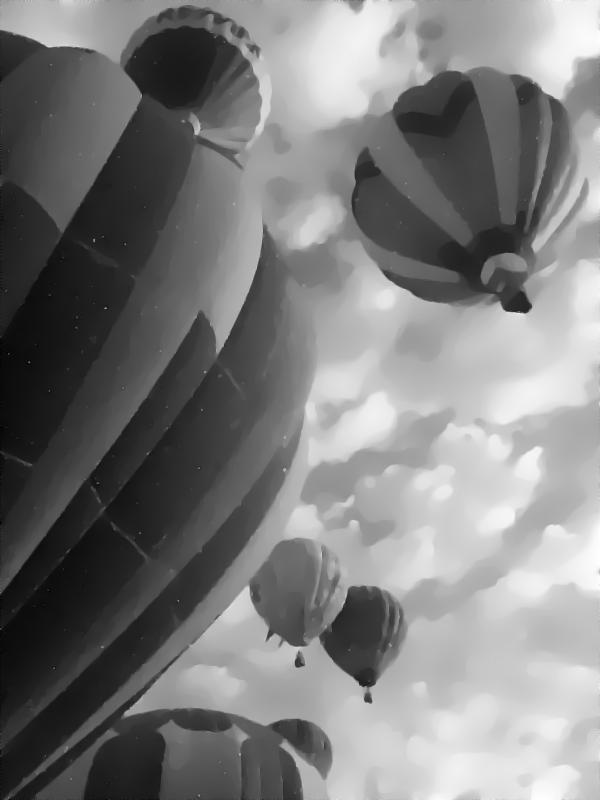
\includegraphics[width=6cm]{tv_denoised_baloons_resized_bw.jpg}
% \caption{The solution of \eqref{tv_images:diffusion_flow}, found using a first order Euler step in time and centered differences in space.}
% \label{fig:tv_image_denoised}
% \end{figure}







